\def\fileversion{v2.25a} \def\filedate{2009/10/10}
%% Package and Class "uiucthesis2009" for use with LaTeX2e.
\documentclass[edeposit,fullpage,draftthesis]{uiucthesis2009}

\usepackage[letterpaper, margin=1in]{geometry}
\usepackage{graphicx}
\usepackage{amsmath}

\usepackage[numbers, square, sort]{natbib}

\usepackage{hyperref}
\usepackage[toc,page]{appendix}

% thai character stuff
\usepackage[thai,english]{babel}
\usepackage[utf8x]{inputenc}

% Hack into CJKutf8 package for an option clash error
%\makeatletter
%\@namedef{opt@inputenc.sty}{utf8}
%\makeatother
%\usepackage{CJKutf8}

\begin{document}

\title{Substrate-Mediated Modulations of Graphene's Electronic Properties}
\author{John Henry Hinnefeld}
\department{Physics}
\phdthesis
\advisor{Nadya Mason}
\degreeyear{2016}
\committee{
Professor S. Lance Cooper, Chair\\
Associate Professor Nadya Mason, Director of Research\\
Associate Professor Lane Martin, University of California, Berkeley\\
Professor Emeritus Richard Weaver}
\maketitle

\frontmatter

%% Create an abstract that can also be used for the ProQuest abstract.
%% Note that ProQuest truncates their abstracts at 350 words.
\begin{abstract}
This is a comprehensive study of caffeine consumption by graduate
students at the University of Illinois who are in the very final
stages of completing their doctoral degrees. A study group of six
hundred doctoral students\ldots.
\end{abstract}

%% Create a dedication in italics with no heading, centered vertically
%% on the page.
\begin{dedication}
To my family.

\foreignlanguage{thai}{\textthai{หนังสน้อยือี}}

\end{dedication}

%% Create an Acknowledgements page, many departments require you to
%% include funding support in this.
\chapter*{Acknowledgments}

This project would not have been possible without the support of
many people. Many thanks to my adviser, Lawrence T. Strongarm, who
read my numerous revisions and helped make some sense of the
confusion. Also thanks to my committee members, Reginald Bottoms,
Karin Vegas, and Cindy Willy, who offered guidance and support.
Thanks to the University of Illinois Graduate College for awarding
me a Dissertation Completion Fellowship, providing me with the
financial means to complete this project. And finally, thanks to
my husband, parents, and numerous friends who endured this long
process with me, always offering support and love.

%% The thesis format requires the Table of Contents to come
%% before any other major sections, all of these sections after
%% the Table of Contents must be listed therein (i.e., use \chapter,
%% not \chapter*).  Common sections to have between the Table of
%% Contents and the main text are:
%%
%% List of Tables
%% List of Figures
%% List Symbols and/or Abbreviations
%% etc.

\setcounter{tocdepth}{4}

\tableofcontents
\listoftables
\listoffigures

%% Create a List of Abbreviations. The left column
%% is 1 inch wide and left-justified
\chapter{List of Abbreviations}

\begin{symbollist*}
\item[CA] Caffeine Addict.
\item[CD] Coffee Drinker.
\end{symbollist*}

%% Create a List of Symbols. The left column
%% is 0.7 inch wide and centered
\chapter{List of Symbols}

\begin{symbollist}[0.7in]
\item[$\tau$] Time taken to drink one cup of coffee.
\item[$\mu$g] Micrograms (of caffeine, generally).
\end{symbollist}

\mainmatter
\chapter{Introduction}

    \section{Motivation}
    \section{Statement of thesis problem}


\chapter{Background}

    Since its initial isolation in 2004 graphene has been the subject of intense research interest. 
    The following chapter presents a summary of the relevant properties and research results 

    \section{Introduction to graphene}

    Much of graphene's interesting behavior comes from its unique, two-dimensional structure. As illustrated in Figure \ref{fig:lattice}, graphene is composed of carbon atoms in a hexagonal lattice. The hexagonal lattice contains two interlaced triangular lattices, labelled \textbf{A} and \textbf{B}. Each individual sublattice has unit vectors $a_1$ and $a_2$. The Brillouin zone of graphene's lattice is also illustrated in Figure \ref{fig:lattice}; the corners, indicated by the labels \textbf{K} and \textbf{K'} are referred to as Dirac points for reasons described below. 
\note{fix this}
    This unique structure gives graphene  a variety of interesting characteristics, however a complete description of its attributes is beyond the scope of this report. Those properties of graphene which are relevant to the proposed research are summarized below; for a more complete description of graphene please see one of the existing review articles \cite{Geim2007}, \cite{CastroNeto2009}. Here I discuss graphene's band structure, the unique variant of the quantum Hall effect this band structure gives rise to, and the possibility of observing this quantum Hall effect in zero magnetic field due to strain effects as well as the general effects of strain on graphene's electronic properties.

    \begin{figure}
    \centering
    \includegraphics{images/background/ElecPropertiesFig2.png}
    \caption[The lattice structure of graphene and its Brillouin zone]{The lattice structure of graphene and its Brillouin zone. Left: Graphene is composed of two interlaced triangular sublattices, labelled \textbf{A} and \textbf{B}. Each sublattice has unit vectors $a_1$ and $a_2$. Right: The Brillouin zone of graphene has several high symmetry points. In particular, the points \textbf{K} and \textbf{K'} are referred to as Dirac points. Adapted from \cite{CastroNeto2009}.}
    \label{fig:lattice}
    \end{figure}
		
	\subsection{Band structure}
    The band structure of graphene is shown in Figure \ref{fig:bandstructure}; undoped graphene is a zero-gap semiconductor. This band structure is calculated using a simple tight-binding model, with a Hamiltonian (using units where $\hbar=1$) \cite{CastroNeto2009}:
    $$
    H = - t \sum\limits_{\langle i,j\rangle,\sigma} (a_{\sigma,i}^\dagger b_{\sigma,j} + \text{H.c.})
    - t' \sum\limits_{\langle\langle i,j\rangle\rangle,\sigma} (a_{\sigma,i}^\dagger a_{\sigma,j} + b_{\sigma,i}^\dagger b_{\sigma,j} + \text{H.c.})
    $$
    where $t$ is the nearest neighbor hopping amplitude, $t'$ is the next nearest neighbor hopping amplitude, and $a_{\sigma,i}$ is the annihilation operator for an electron of pseudo-spin $\sigma$ at position $i$ on sublattice \textbf{A}. The Hermitian conjugate $a^\dagger$ gives the creation operator, and the $b$ operators are similarly defined for the \textbf{B} sublattice. This Hamiltonian yields an energy spectrum of the form \cite{CastroNeto2009}:

    $$
    E(\mathbf{k}) = \pm t \sqrt{3 + f(\mathbf{k})} - t' f(\mathbf{k}) \;\;\; \text{with} \;\;\;
    f(\mathbf{k}) = 2 \cos{\sqrt{3} k_y a } + 4 \cos{\frac{\sqrt{3}}{2} k_y a} \cos{\frac{3}{2} k_x a}
    $$

    \begin{figure}
    \centering
    \includegraphics[width=0.4\textwidth]{images/background/ElecPropertiesFig3.png}
    \caption[The band structure of graphene]{The band structure of graphene. At the corners of the Brillouin zone the upper and lower bands meet. Near these points, known as Dirac points, the dispersion relation is approximately linear. Adapted from \cite{CastroNeto2009}.}
    \label{fig:bandstructure}
    \end{figure}


	\subsection{Dirac fermions}
    In the low energy regions near the corners of the Brillouin zone the dispersion relation for graphene is approximately linear, as indicated in Figure \ref{fig:bandstructure}. That is, for electrons or holes near these points,
    $$
    E = \hbar v_F \sqrt{k_x^2 + k_y^2}
    $$
    (where $k_x$ and $k_y$ are measured from the corner point) which has the same form as the energy of a massless, relativistic particle governed by the Dirac equation. These points are therefore called Dirac points, and in their vicinity the electrons behave as massless Dirac fermions. Each corner of the hexagonal Brillouin zone is related to two others by a reciprocal lattice vector, therefore two of the Dirac points, typically labelled $K$ and $K'$ are inequivalent.

    The linear dispersion relation is not the only factor which ties transport in graphene to the Dirac equation; the two-component wavefunction of pseudoparticles in graphene is analogous to the spinor wavefunction used to describe spin $\frac{1}{2}$ particles in the Dirac equation \cite{Katsnelson2006}. In graphene the two components correspond to the contributions to the pseudoparticle wavefunction from each of the two sublattices, whereas in quantum electrodynamics (QED) the spinor accounts for the spin up and spin down components of the wavefunction.

	\subsection{Quantum Hall effect}
    Graphene displays a unique variant of the quantum Hall effect (QHE) due to the massless, Dirac fermion nature of its charge carriers \cite{Novoselov2005}, \cite{Zhang2005}, as seen in Figure \ref{fig:QHEinG}. In typical materials the application of a large magnetic field leads to the formation of Landau levels (LLs), which when successively filled by increasing the carrier concentration yield plateaux in the Hall conductivity at $\sigma_{xy} = \pm (4e^2/h) N$ where $N$ is an integer. Additionally, in typical materials there is no Landau level at $E=0$, due to the $E=\hbar \omega_c (n + 1/2)$ energy quantization of massive particles in a magnetic field, therefore the first plateaux appear at $\pm 4 e^2/h$. The quantum Hall effect as observed in graphene differs from the standard, integer QHE in two ways: the plateaux are shifted by $2 e^2/h$ and the sequence is uninterrupted as it passes through zero carrier density. Both differences stem from the massless character of graphene's charge carriers.

    For massless particles in a magnetic field, such as the Dirac fermions in graphene, the energy quantization is $E = [ 2 e \hbar {c\ast}^2 B (N + 1/2 \pm 1/2) ]^{1/2}$ \cite{Novoselov2005}, where the sign of the last term depends on the pseudospin (or sublattice index) of the particle. This has two consequences; first, when $\pm \rightarrow -$ this quantization admits an $E=0$ Landau level, which in turn causes the sequence of plateaux in the Hall conductivity to be uninterrupted as it passes through zero carrier density. Second, the $E=0$ Landau level admits only those particles with `minus' pseudospin polarization, therefore it is half as degenerate as all other LLs. This accounts for the $1/2$ offset in the locations of the Hall conductivity plateaux in graphene, $\sigma_{xy} = (4 e^2/h )(N + 1/2)$.

    An additional consequence of the masslessness of charge carriers in graphene is the persistence of quantum Hall effects to room temperature \cite{Novoselov2007}. Considering again the energy quantization for Dirac fermions in a magnetic field quoted above, for $c\ast = v_F \approx 10^6$ m $s^{-1}$ a 45 T field yields an energy gap of $\approx$ 2400 K between the $N=0$ and $N=\pm1$ Landau levels, an order of magnitude greater than thermal fluctuations at room temperature. The high carrier concentration and temperature-independent carrier mobility also contribute to the robustness of the effect \cite{Novoselov2007}.

    \begin{figure}
    \centering
    \includegraphics[width=0.45\textwidth]{images/background/QHEinG.png}
    \caption[The quantum Hall effect in graphene]{The quantum Hall effect in graphene. The Hall conductivity and longitudinal resistivity are plotted as a function of carrier concentration. Hall plateaux are present at $4 e^2 / h (N + 1/2)$, offset from the expected values by $2 e^2 / h$, and continue uninterrupted through zero concentration. Inset: Hall conductivity versus carrier concentration for bilayer graphene, showing the expected characteristics of the integer quantum Hall effect for comparison. Adapted from \cite{Novoselov2005}.}
    \label{fig:QHEinG}
    \end{figure}

        
    \section{Doping graphene}
    
        \subsection{Electrostatic gating}
        
        \subsection{Chemical adsorbates}
    
        \subsection{Substrate effects in graphene}
        The substrate used to support graphene strongly affects electrical transport in the graphene. Scattering by surface phonons at the SiO$_2$ interface has been shown to limit the room temperature mobility of graphene \cite{Chen2008}, and scattering by charge impurities is responsible for the asymmetry between electron and hole conductivities \cite{Hwang2007}. Charge impurities can also create inhomogeneities in graphene's local carrier density, which are thought to be responsible for the saturation of conductivity at low carrier densities \cite{Hwang2007}. Substrate features can also cause delamination of the graphene from the substrate; previous work has observed a snap-through transition for multilayer graphene on corrugated substrates \cite{Scharfenberg2012} as well as the formation of network of wrinkle delaminations on a substrate decorated with silica nanoparticles \cite{Yamamoto2012}.
    
        Certain experiments, in an attempt to minimize the effect of the substrate have fabricated devices using suspended graphene \cite{Bolotin2008}, \cite{Du2008}. In a particularly noteworthy example, the authors of ref \cite{Bolotin2008} observed carrier mobilities of up to 200,000 cm$^2$ V$^{-1}$ s$^{-1}$, an order of magnitude greater than the best results for graphene on silicon substrates, showing that the substrate can have a distinct impact on graphene's electrical properties. Recently several groups have also begun fabricating graphene devices on hexagonal boron nitrides (hBN) substrates, where the atomically flat surface, large bandgap, and similar lattice constant to graphene yield drastically improved electronic properties compared to samples fabricated on SiO$_2$ substrates \cite {Dean2010}, \cite{Xue2011}.
    
        Alternatively, strong substrate interactions can also be used to deliberately tune graphene's electrical properties. In particular, functional ferroelectric substrates such as PbZr$_{0.2}$Ti$_{0.8}$O$_3$ (PZT) have been shown to vary carrier type and density in graphene with varying substrate polarizations \cite{Baeumer2013}, as seen in Figure \ref{fig:GonPZT}. This effect is bidirectional: application of a large bias to the graphene can also flip the polarization of the underlying PZT.
    
            %\begin{wrapfigure}[25]{R}{0.50\textwidth}
            \begin{figure}
            \centering
            \includegraphics[width=0.35\textwidth]{images/background/ChristophDevice.png}
            \includegraphics[width=0.45\textwidth]{images/background/ChristophFig4.png}
            \caption[Graphene on ferroelectric substrates]{Left: A graphene FET fabricated on a PZT substrate. Right: Variable carrier type in a graphene FET on a ferroelectric substrate. I-V sweeps are shown for for the same device after gate voltage pulses are applied to switch the polarization of the ferroelectric layer. Adapted from \cite{Baeumer2013}.}
            \label{fig:GonPZT}
            \end{figure}
        
        
    \section{Straining graphene}
    
        \subsection{Graphene's mechanical strength}
    
        \subsection{Band gap engineering}
        Several research groups have considered, both experimentally \cite{Ni2008}, \cite{Kim2009}, \cite{Mohiuddin2009}, \cite{Zang2013} and theoretically \cite{Pereira2009}, \cite{Low2011}, the effect of uniaxial strain on graphene. A number of results are consistent between groups. First, the effect of uniaxial strain on the electronic properties of graphene can be observed through Raman spectroscopy; in ref \cite{Ni2008} the authors observe shifts in the G and 2D band peaks of -27.8 and -14.2 cm$^{-1}$ / percent strain respectively, confirming the interactivity of strain and graphene's electronic properties as well as offering a method to locally measure the strain applied to graphene.
    
        Second, uniaxial strain is predicted to open a gap in the band structure, either by itself at high strains \cite{Pereira2009} or in conjunction with a correlated scalar potential \cite{Low2011}. Experimental work following the latter approach observed an increasing sheet resistivity with decreasing temperature in a graphene device patterned atop lithographically defined corrugations on a SiO$_2$ substrate \cite{Lee2013}. This behavior is indicative of a gap in the band structure, which the authors calculate to be approximately 200 meV. In this case the periodic potential comes from the periodic, substrate-induced doping in the regions not covered by the corrugations.
    
        \subsection{Pseudomagnetic fields}
        Recent work, both theoretical \cite{Guinea2009} and experimental \cite{Levy2010}, \cite{Yan2012} suggests that non-uniform strains in graphene have an effect similar to an applied magnetic field. From a theoretical perspective these strain-induced pseudomagnetic fields stem from a modification of the nearest and next nearest neighbor hopping amplitudes; as the lattice is strained the distances between lattice sites vary, and with them the relevant hopping amplitudes $t$ and $t'$. This strain effect can be modeled by introducing a gauge field vector potential, which has an effect similar to that of a magnetic vector potential field. However, unlike an actual magnetic field a strain-generated pseudomagnetic field has a different sign for charge carriers in the \textbf{K} and \textbf{K'} Dirac points, and therefore does not violate time reversal symmetry \cite{Guinea2009}.
    
        These pseudomagnetic fields are predicted to be on the order of tens of tesla. Such high fields, in conjunction with graphene's high carrier concentration and mobility, offer the potential to observe a zero field quantum Hall effect. A key requirement in generating pseudomagnetic fields is that the strain profile be anisotropic; to date experimental efforts have focused on strain created by nanobubble \cite{Levy2010} or nanoridge \cite{Yan2012} defects. However defect-oriented experimental design schemes yield extremely small areas of graphene under strain, and as such the strain-related physics is only accessible through scanning tunneling microscopy (STM) measurements. Therefore in order to observe macroscopic transport effects like a zero field quantum Hall effect I propose a device scheme with arrays of patterned strain-inducing features.



\chapter{Experimental Techniques}

    This thesis describes the results of experimental work, and while the experimental results comprise the bulk
    of this work's novelty a thorough record of the the experimental methods employed to produce those results 
    is crucial for future reproducibility.
    In this chapter I present a summary of the fabrication, characterization, and measurement techniques used
    in the course of this research.
    
    \section{Sample Fabrication}
    
        Sample fabrication is the primary task for experimental work on graphene devices. 
        In this section I present the experimental techniques used to fabricate graphene devices.
    
        \subsection{Graphene synthesis and transfer}
        
        
            \subsubsection{Mechanical exfoliation}
            
            There are two widely used methods used to produce graphene for 
        experimental research: mechanical exfoliation\cite{novoselov2004electric} and chemical vapor
        deposition (CVD) growth\cite{li2009large}. In mechanical exfoliation highly ordered
        pyrolitic graphite is repeatedly cleaved, typically by attaching and 
        then peeling off Scotch tape. After a succession of such cleaving steps
        small regions of monolayer graphene are left attached to the Scotch
        tape, which are then transferred to a silicon wafer having a 300nm
        thick layer of SiO$_2$. An optical interference effect caused by the 
        combination of the oxide layer and the graphene allows the graphene
        regions to be identified with an optical microscope \cite{Blake2007}.
        This process is illustrated schematically in Figure \ref{fig:exfoliation}.
        Mechanical exfoliation produces the highest quality graphene as
        measured by electron mobility; values up to 60,000 cm$^2$ V$^{-1}$
        s$^{-1}$ have been reported \cite{Dean2010}. However, the size of the 
        resulting graphene flakes is limited, typically to tens of square
        microns, and the transfer process precludes any alignment of graphene
        with pre-existing substrate features.
        
            \begin{figure}
            \centering
            \includegraphics[width=0.6\linewidth]{images/experimentaltechniques/exfoliation.png}
            \caption[Mechanical exfoliation of graphene]{
                \textbf{(a-b)} Highly ordered pyrolitic graphite is cleaved using Scotch tape.
                \textbf{(c)} The cleaved graphite is pressed onto the target substrate.
                \textbf{(d)} The Scotch tape is peeled off the target substrate, leaving a monolayer of graphene.
                Image adapted from \cite{novoselov2012two}}
            \label{fig:exfoliation}
            \end{figure}

        
            \subsubsection{CVD growth}

            In the CVD growth process a metal foil, usually nickel or copper, is
        placed in a vacuum furnace and heated while H$_2$ and CH$_4$ are 
        introduced at controlled rates and for controlled times. Properly
        optimized growth recipes will yield uniform, monolayer graphene on
        top of the metal foil \cite{reina2008large, kim2009large, li2009large, li2009transfer}. 
        For the precise recipes used to grow the graphene used in this research see Appendix \ref{appendix:fab}.
        
        Unlike graphene produced by mechanical
        exfoliation, CVD graphene usually (though not always, see 
        \cite{Petrone2012}) has multiple domains \cite{Li2010} which accounts
        for its lower quality, again as measured by electron mobility. Typical
        values for CVD graphene are in the $10^3$ to $10^4$ cm$^2$ V$^{-1}$
        s$^{-1}$ range \cite{Petrone2012}. From a practical perspective, the 
        disadvantage of CVD graphene's limited mobility
        is counter-balanced by the ease and volume of production via this method:
        while exfoliated graphene flakes are limited to tens of square microns, 
        CVD graphene has been grown in 30 inch-wide films\cite{bae2010roll}.
        Larger graphene films allow for entire substrates to be covered, which 
        in turn allows for device designs where graphene is deposited atop existing
        substrate features.
        
            \subsubsection{Wet transfer}
            
            Graphene grown on metal foils by chemical vapor deposition must be transferred to 
        an insulating substrate before its electrical properties can be measured.
        This transfer is a critical step: if done poorly it has the potential to 
        drastically alter the properties of the graphene, whether by destroying
        the mechanical integrity of the graphene or by introducing substantial electrical doping.
        Transferring graphene onto flexible or patterned substrates introduces additional
        complexities. 
        
        \begin{figure}
            \centering
            \includegraphics[width=0.8\linewidth]{images/experimentaltechniques/wettransfer.png}
            \caption[Mechanical exfoliation of graphene]{
                `Wet transfer' of CVD graphene.
                Image adapted from \cite{kumar2013synthesis}}
            \label{fig:wettransfer}
            \end{figure}

        The simplest transfer procedure is illustrated schematically in Figure \ref{fig:wettransfer}.
        Copper foil with CVD graphene grown on top is coated with a thin, sacrifical layer of the 
        polymer poly(methyl methacrylate) (PMMA) and then placed in a chemical
        bath to etch away the metal. Once the metal is removed the PMMA-coated graphene 
        remains floating on the surface of the solution. The solvent is then flushed and replaced
        with de-ionized water.
        Finally the floating graphene / PMMA stack can be
        scooped onto the desired substrate, at which point the PMMA is removed using acetone
        \cite{reina2008large, kim2009large, li2009large}.
        
        
        This method produces large graphene
        sheets (limited only by the size of the vacuum furnace, on the order of
        1 cm$^2$ in most cases), and by covering the entire substrate offers
        the possibility of aligning graphene with substrate features. However,
        the transfer process can degrade the graphene by introducing chemical
        dopants and mechanical defects.
        
            
            \subsubsection{Copper transfer}
            Graphene was grown using established chemical vapor deposition (CVD) techniques \cite{Li2009}, and then transferred to a copper-coated silicon wafer where it was patterned using photolithography and reactive ion etching. Next, a piece of PDMS was mechanically pressed onto the silicon wafer, and the copper was then etched to leave patterned graphene on the PDMS substrate\cite{Lee2010}.
            
            \subsubsection{Critical point drying transfer}
            
            
        \subsection{Substrate patterning}
            \subsubsection{Lithography}
            \subsubsection{Deposition}
            \subsubsection{Reactive ion etching}
    
    \section{Sample Characterization}
    The primary challenge of experimental condensed matter research, at least as measured by graduate student effort, lies in fabricating working devices. The fabrication techniques described above require finesse, skill, and a certain degree of luck (especially when working with temperamental equipment). As such, a substantial fraction of the fabricated devices will fail to work. Characterizing the different failure modes of a given fabrication process -- and thereby determining the optimal process parameters -- is a crucial part of each research project. In this section several techniques which effectively characterize the quality and physical integrity of graphene and other fabricated device elements are described.
    
    \note{mostly about checking quality and integrity of graphene}
        \subsection{Atomic Force Microscopy}
        \subsection{Scanning Electron Microscopy}
        \subsection{Raman Spectroscopy}
            \subsubsection{Characterizing Defects and Number of Layers}
            \subsubsection{Characterizing Doping and Strain}
    
    \section{Data collection}
        \subsection{Transport Measurements}
            \subsubsection*{Two-Point Measurements}
            \subsubsection*{Four-Point Measurements}
            \subsubsection*{Hall Measurements}
        \subsection{Raman Spectroscopy Mapping}
    
    
\chapter{Results and Discussion}

\section{Graphene on flexible substrates}
Recent advances in graphene production \cite{Kim2009, Bae2010, Lee2010} have enabled the fabrication of a variety of flexible, graphene-based electronic components, including transparent interconnects \cite{Kim2011}, high-performance capacitors \cite{El-Kady2012}, and transistors \cite{Lee2011}. The prospect of flexible, graphene-based electronic devices suggested by these results raises an important question: are graphene's electrical properties and mechanical integrity robust under the strains graphene is likely to experience in such devices? Pristine graphene has an exceptionally high breaking strength \cite{Lee2008}, yet it may be susceptible to ripping, particularly if it has defects \cite{Kim2012} and/or strong  surface adhesion \cite{Sen2010}. It is still relatively unknown under what strain conditions substrate-supported graphene rips, and how the electrical properties are then altered.

In this section I describe the results of a research project wherein atomic force microscopy (AFM) and electrical transport measurements were combined to study the effects of lateral strain on rips in graphene. We find that graphene adhered to a flexible substrate and then stretched laterally can develop small rips with only 1\% applied strain. However, even with ripping, the electrical properties remain relatively robust: introducing small rips slightly increases the resistance, but subsequent strain-relaxation cycles over the same strain range change transport only modestly, and in a largely reversible fashion. Such resilience is atypical for conducting thin films, which typically demonstrate rapid and irreversible device failure after the onset of rip formation \cite{Cairns2000,Fortunato2002}.

    \subsection{Device configuration}
    
    Devices consisted of patterned graphene placed on flexible polydimethylsiloxane (PDMS) substrates. The devices were fabricated using a modified transfer printing process, similar to that described in Ref \cite{Kim2009}. Graphene was grown using established chemical vapor deposition (CVD) techniques \cite{Li2009}, and then transferred to a copper-coated silicon wafer where it was patterned using photolithography and reactive ion etching. Next, a piece of PDMS was mechanically pressed onto the silicon wafer, and the copper was then etched to leave patterned graphene on the PDMS substrate \cite{Lee2010}. Raman spectroscopy was used to confirm the presence of graphene on the PDMS as shown in Figure 1c; the shape of the Raman 2D peak \cite{Ferrari2006}, as well as subsequent AFM measurements verified the single-layer character of the graphene. Finally, shadow-mask evaporation was used to deposit Ti/Au contact pads. The device geometry is illustrated in Figure 1a: a narrow graphene bridge connects two large graphene pads, each of which is covered with a Ti/Au contact pad. We studied 13 different devices having bridge aspect ratios ranging from 1.5:1 to 12:1 (length:width) and widths of 100, 50, and 25 $\mu$m. The data in this manuscript focuses on a device with a bridge width of 25 $\mu$m and an aspect ratio of 2:1. The data for all samples yielded similar qualitative results. Quantitative differences in transport data between different devices seemed to be uncorrelated with the bridge dimensions, and were instead dominated by pre-existing rips in the graphene, which are often introduced during the graphene transfer process \cite{Kim2012}. Graphene produced by CVD is known to be polydomain, but it has been shown that rips in graphene do not preferentially follow grain boundaries \cite{Kim2012}.
    
    Transport and AFM measurements were performed while the PDMS substrate was mounted in a mechanical stretching stage, as shown in Figure 1b. The substrate was clamped at either end, and then strained by turning the threaded rod, which laterally moves the sliding clamp along its guide rails. A mechanical stepper motor was used to control the stretching stage position to ensure reproducibility. Variable device positioning on the substrate as well as slight variations in substrate thickness preclude exact conversion between strain applied to the substrate and to the device, therefore strain values reported in this work are given in `turns of the stretching stage control rod'. Each turn strains the substrate by approximately one percent, and we estimate that the strain applied to the graphene differs from that applied to the PDMS substrate by no more than ten percent. However, our conclusions are unaffected by this uncertainty, as variations in the magnitude of applied strain between devices only shift the strain axis of the data while preserving the observed trends. Transport measurements were performed by placing micro-manipulator probes in contact with the gold contact pads at each strain value, and AFM measurements were performed with an Asylum Research MFP-3D.
    
    \subsection{Resistance changes under uniaxial strain}
    
    Typical electrical transport vs. strain data is shown in Figure 2. Figure 2a demonstrates three important features of the data: first, during the initial application of strain (A to B in the Figure) the resistance increases (for this sample, by approximately 43 percent). Typical values for this initial increase in other devices ranged from 20 to 40 percent of the starting resistance. Second, the resistance of the device decreases as the applied strain is relaxed (from B to C) by 7 percent for this device, and typically by between 6 and 14 percent. Finally, in subsequent strain-relaxation cycles over the same strain range the resistance changes only moderately, and in a largely reversible fashion. This reversibility is further demonstrated in Figure 2b; data from the same device recorded during the third, fourth, and fifth strain-relaxation cycles are shown in green, blue, and red respectively. In each case the resistance changes by $\sim$14\% for $\sim$3\% applied strain, and returns to within 8\% of its original value. This behavior -- an increase in resistance with the initial application of tensile strain, followed by moderate and reversible changes in the resistance during subsequent strain-relaxation cycles over the same strain region -- persists up to approximately 15\% applied strain, at which point the devices become permanently non-conducting.

    \begin{figure}
    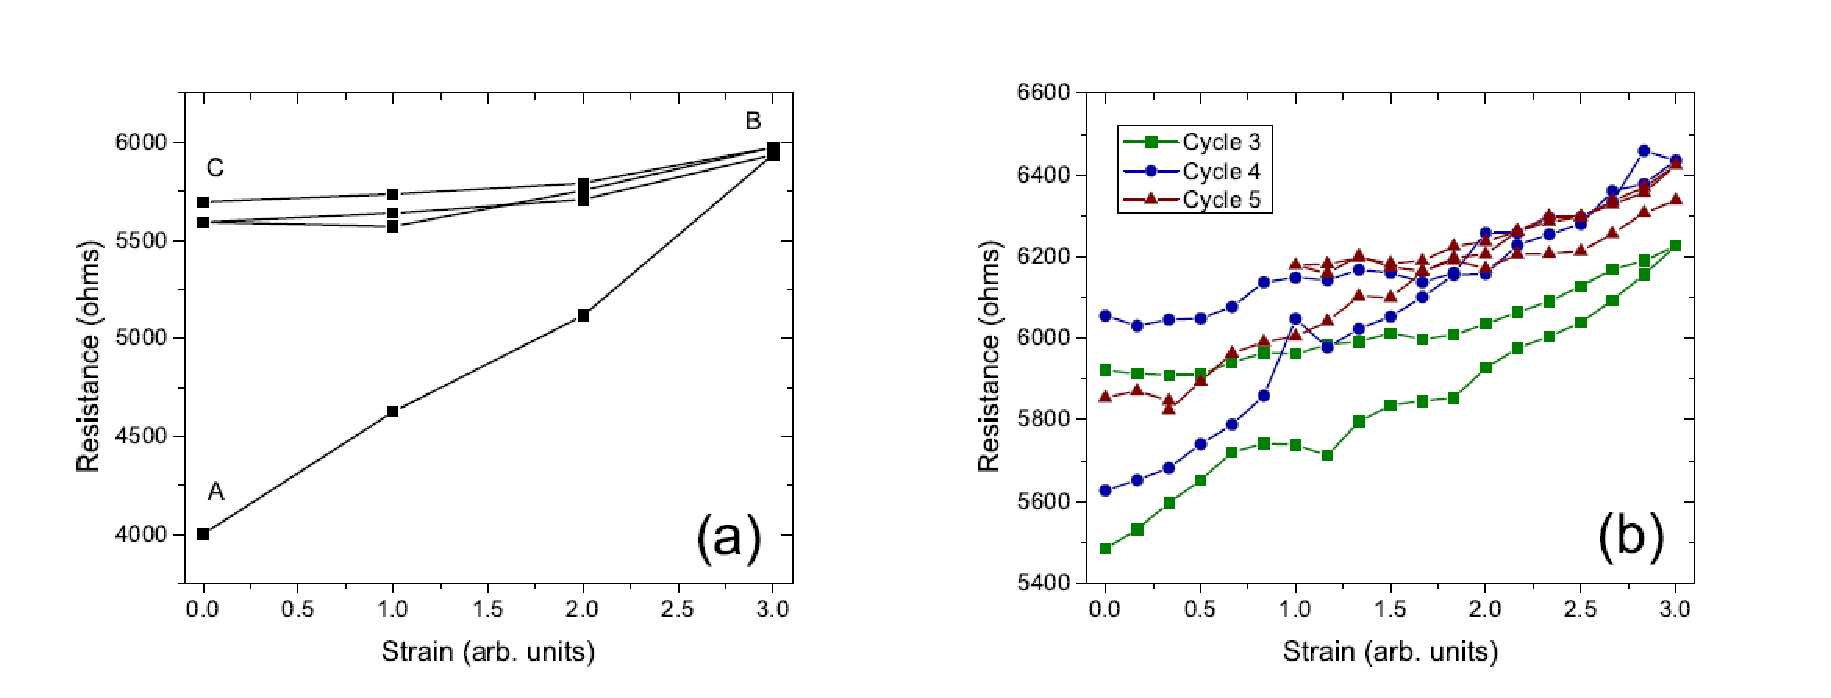
\includegraphics[width=\linewidth]{images/resultsanddiscussion/rippingpaper-RvsStrain.eps}
    \caption[Resistance vs Strain for graphene on flexible substrates]{\textbf{(a)} Electrical resistance of a graphene device vs. applied tensile strain. The initial application of strain significantly increases the resistance while subsequent strain-relaxation cycles over the same strain range yield smaller, mostly reversible changes in the resistance. \textbf{(b)} Three consecutive strain-relaxation cycles (Cycles 3,4,5), showing largely reversible transport characteristics. Three arb. units correspond roughly to three percent applied strain.}
    \label{fig:rippingpaper-RvsStrain}
    \end{figure}

    \subsection{Rip formation under strain}

\section{Graphene on ferroelectric substrates}
    \subsection{Device configuration}
    \subsection{Variable local doping via substrate modifications}
    \subsection{Hysteresis in local doping}
    \subsection{Polar adsorbates as local dopants}

\section{Graphene on strain array substrates}
    \subsection{Device configuration}


\chapter{Summary and conclusions}
\section{Summary of results}
\section{Future work}

\begin{appendices}

\chapter{Device Fabrication Procedures}
\label{appendix:fab}
\section{Graphene on flexible substrates}
\section{Graphene on ferroelectric substrates}
\section{Graphene on strain array substrates}

\chapter{Python Measurement Code}
\section{Instrument Drivers}
\section{Gate-sweep Example}
\section{Field-sweep Example}
\section{Sheet Resistance Example}

\end{appendices}

\backmatter

\bibliographystyle{catunsrt}
\bibliography{rippingpaper,pztpaper,PrelimPaper,thesis}


\end{document}
\endinput
